\documentclass[10pt]{article}         %% What type of document you're writing.

%%%%% Preamble

%% Packages to use

\usepackage{amsmath,amsfonts,amssymb}   %% AMS mathematics macros
\usepackage{graphicx}
\usepackage{subfig}
\usepackage{lmodern}  % for bold teletype font
\usepackage{amsmath}  % for \hookrightarrow
\usepackage{xcolor}   % for \textcolor
\usepackage{listings}
\usepackage{mathtools}
\lstset{
  basicstyle=\ttfamily,
  columns=fullflexible,
  frame=single,
  breaklines=true,
  postbreak=\mbox{\textcolor{red}{$\hookrightarrow$}\space},
}

%% Title Information.

\title{HomeWork 05}
\author{Deep Dand}
%% \date{2 July 2004}           %% By default, LaTeX uses the current date

%%%%% The Document

\begin{document}

\maketitle

\begin{abstract}
Kmeans and MLP experiments
\end{abstract}

\section{Problem 1}
\subsection{e}
The code below was run for different values of n\_colors between $2-64$. 

Code Begins
\lstinputlisting{hw5.kmeans.img.py}
Code ends
\\Output\\
As it is seen in the images above, as we get close to the colors value 2, the image starts to look more and more funny. As the $n\_colors$ value is closer to 64, the image is reproduced well with more colors.

In the images below, until values of n\_color =15, 16 are the last to show any signs of color and after that as values are reduces, the image gets more and more funny. 
\begin{figure}
\begin{tabular}{cccc}
\subfloat[n\_color=2]{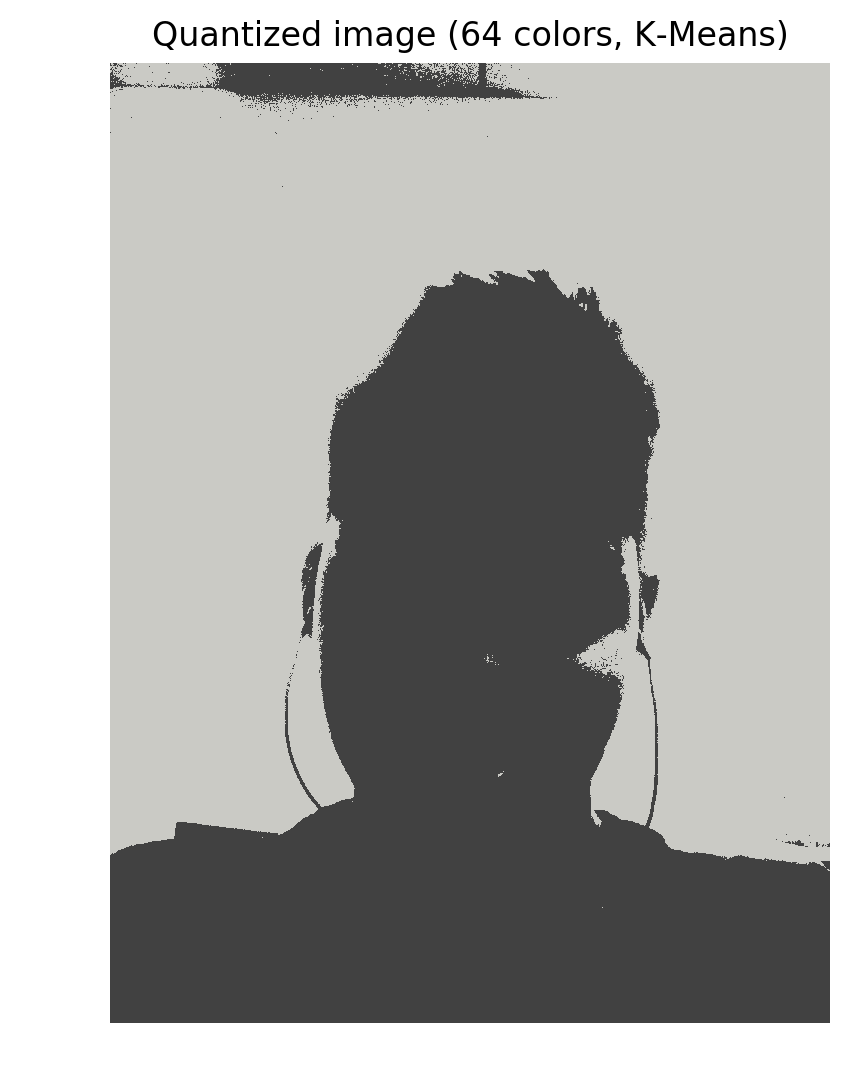
\includegraphics[width = 1.5in]{n_colors_2.png}} &
\subfloat[n\_color=8]{
\includegraphics[width = 1.5in]{n_colors_8.png}} &
\subfloat[n\_color=12]{
\includegraphics[width = 1.5in]{n_colors_12.png}}\\
\subfloat[n\_color=15]{
\includegraphics[width = 1.5in]{n_colors_15.png}} &
\subfloat[n\_color=16]{
\includegraphics[width = 1.5in]{n_colors_16.png}} &
\subfloat[n\_color=32]{
\includegraphics[width = 1.5in]{n_colors_32.png}}\\
\subfloat[n\_color=64]{
\includegraphics[width = 1.5in]{n_colors_64.png}} &
\end{tabular}
\caption{3 x 3}
\end{figure}
\newpage
Ans ii.
\\The other possible applications could be, image compression where we can choose value of n\_color to a value which can represent the image almost equal quality but will eventually take really less pixels to draw it. 


Ans iii.
\\The resulting picture was funny at the end because the less number of colors meaning that pixels in the original picture were replaced by shades of black and white and it makes white brighter in the picture and black darker. All other colors are converted in one or the other shade of gray depending on the n\_colors value. For e.g, if it is 2(the first image in the grid), the image will only be converted in black and white. If the n\-value = 15, it the algorithm has 13 shades of gray and white and black color to represent the whole picture. 

\newpage
\section{Problem 2}
MLP Program. 
\subsection{c}
The code below is run for 1000 samples and the best value of neurons and $\eta$ is noted.
\lstinputlisting{hw5.MLP.sol.py}
Code ends. 
\\Output\\
The screen-shot below shows the result with  
$$ Number\ of\ neurons\ = 23 $$
$$ \eta = 0.1$$
$$ Training\ set\ score\ = 0.8345 $$
$$ Testing\ set\ score = 0.8397 $$
\\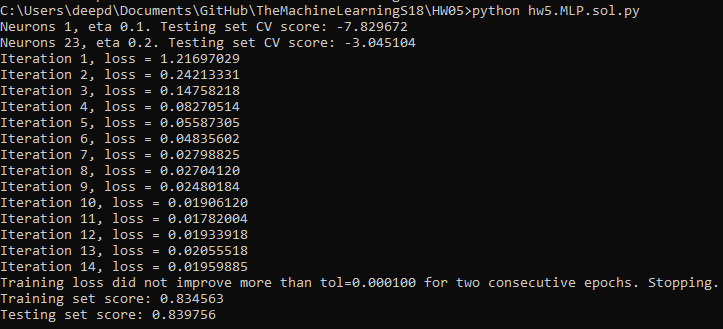
\includegraphics[scale=0.55]{hw51k_n23.PNG}
\\The screen-shot below shows the result with

$$ Number\ of\ neurons\ = 74 $$
$$ \eta = 0.1 $$
$$ Training\ set\ score\ = 0.9012 $$
$$ Testing\ set\ score\ = 0.8813 $$

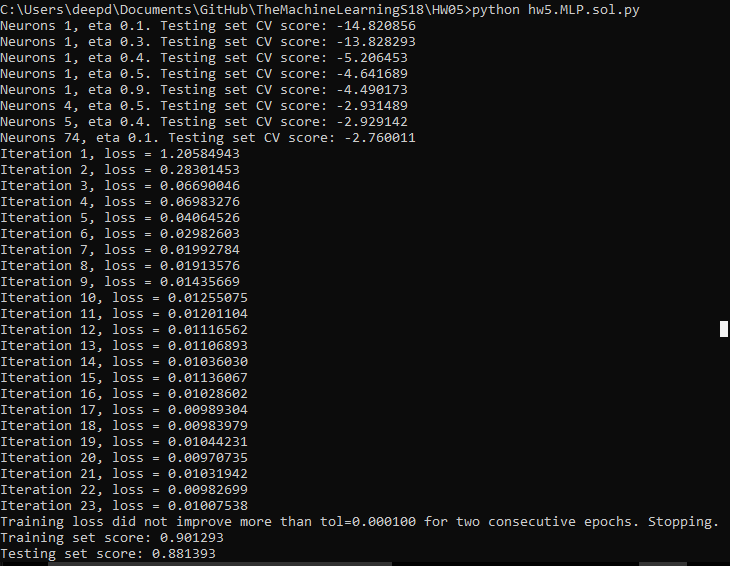
\includegraphics[scale=0.55]{hw51k_n74.PNG}
As seen above, I tried running program two times to see the difference in results and also understand the relationship between number of neurons.
The program is run again with 10000 data points and below is the result for the same.
The output is,
\\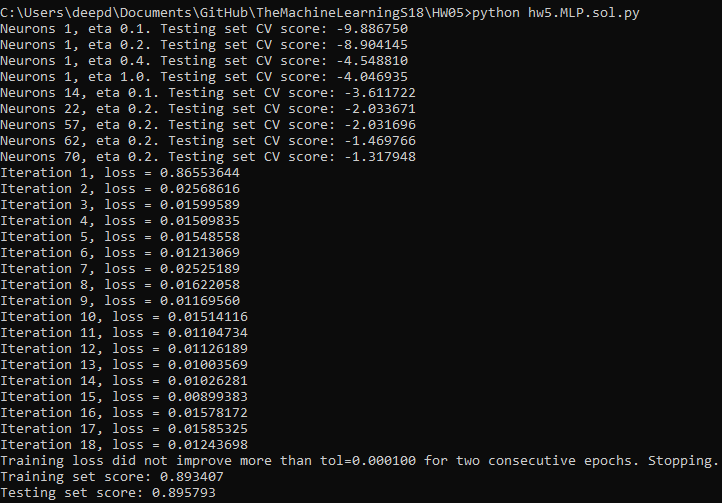
\includegraphics[scale=0.75]{hw5q2d.PNG}
The output graph looks like,
\\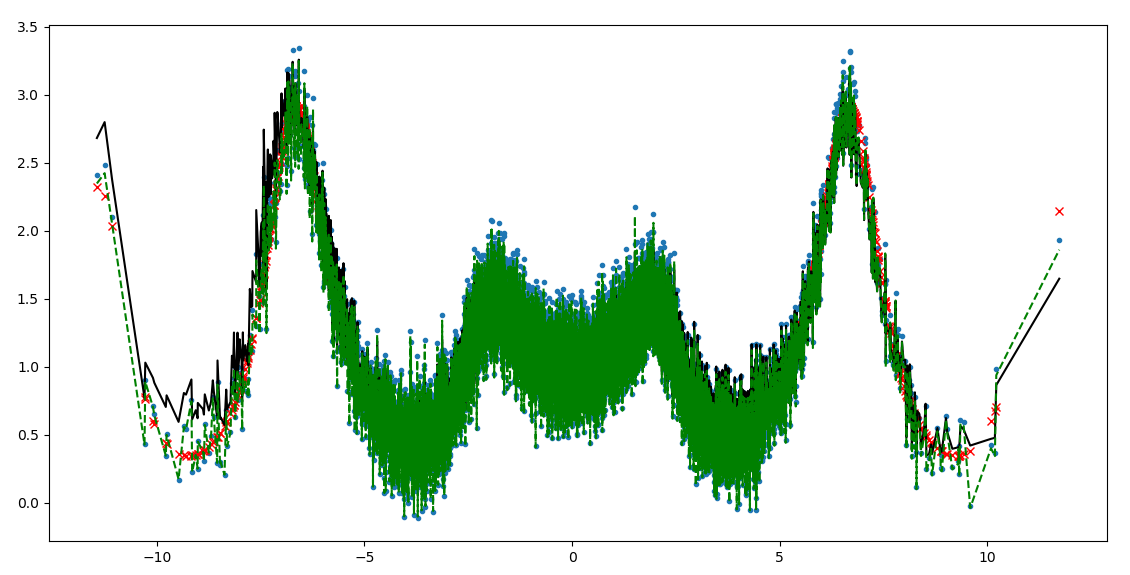
\includegraphics[scale=0.45]{hw5q2d1.PNG}
\\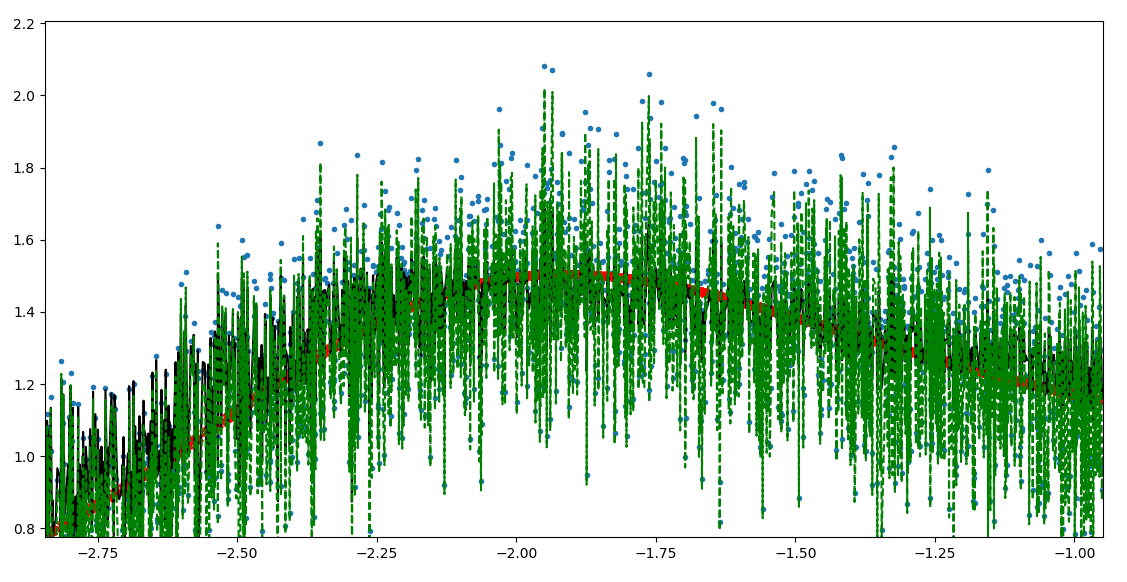
\includegraphics[scale=0.45]{hw5q2d2.PNG}

Question- 
What do you think is happening? What is your interpretation of the
number of neurons with respect to the performance of the network?
\\Answer
\begin{itemize}
\item I think that that the program with $1000$ data points and $10000$ data points have maximum  $\eta = 0.2$  and it produces pretty good results.
\item For this network any value above $0.2$ for $ \eta $ is large and so it stops iterating.
\item As far as number of neurons go, it the two results for $1000$ data points suggest neurons count 23 and 74, there is one more result that I didn't include because it also had neurons count to be 79 with $ \eta = 0.1 $. 
\item With $10000$ data points, it was surprising to see that number of neurons are $70$ which states that for $1000-10000$ data points network performance is almost the same given the number of neurons are in range of 70. 
\end{itemize}
\end{document}

